%===================================
\chapter{Représentation des données\index{Representation des 
         données@Représentation des données}}
%====================================


Nous voici arrivés au terme du cours de logique de
1\textsuperscript{ère} année. Ce chapitre apporte une synthèse des
différentes notions vues tout au long du cours, et propose quelques
pistes de réflexion quant au choix d’une bonne représentation des
données qui se pose lors de la résolution de problèmes de programmation
avancés.

Les exercices de ce chapitre sont essentiellement des questions
d’anciens examens ; comme ces exercices ne sont pas directement liés à
la matière d’un chapitre précis, leur difficulté tient en partie dans
le bon choix d’une représentation des données et de la démarche
algorithmique la plus adéquate à mettre en œuvre pour agir sur ces
données en vue d’obtenir le résultat escompté. Noter que l’efficacité
d’un algorithme est lié étroitement au choix de la représentation.


%======================================
\section{Se poser les bonnes questions}
%=======================================

Revenons à la case départ : nous avons commencé ce cours en situant les
notions de \textbf{problème} et de \textbf{résolution}. Nous avons vu
qu’un problème bien spécifié s’inscrit dans le schéma :

\cadre{
étant donné [les données] on demande [l’objectif]
}

Une fois le problème correctement posé, on peut partir à la recherche
d’une \textbf{méthode de résolution}, c’est-à-dire d’un algorithme en
ce qui concerne les problèmes à résoudre par les moyens informatiques.

Tout au long de l’année, nous avons vu divers modèles et techniques
algorithmiques adaptées à des structures particulières (les nombres,
les chaines, les tableaux, les variables structurées, les objets, les
listes, les fichiers…). La plupart des exercices portaient directement
sur ces structures (par ex. calculer la somme des nombres d’un tableau,
fusionner deux fichiers en un seul, extraire une sous-liste à partir
d’une liste donnée). Ces exercices d’entrainement et de formation
quelque peu théoriques constituent en fait des démarches algorithmiques
de base qui trouvent toutes une place dans des problèmes plus
complexes.

Mais la plupart des problèmes issus des situations de la vie courante
auxquels se confronte le programmeur s’expriment généralement de
manière plus floue : par ex. dresser la comptabilité des dépenses
mensuelle d’une firme, faire un tableau récapitulatif du résultat des
élections par cantons électoraux, faire une version informatique d’un
jeu télévisé… Les exemples sont infinis !


C’est dans le cadre de ce genre de problème plus complexe que se pose le
problème de la \textbf{représentation de données}. Une fois le problème
bien spécifié (par les données et l’objectif) apparaissent
naturellement les questions suivantes : quelles données du problème
sont réellement utiles à sa résolution ?~(Il est fréquent que l’énoncé
d’un problème contienne des données superflues ou inutiles). Y a-t-il
des données plus importantes que d’autres ? (données principales ou
secondaire). Les données doivent-elles être consultées plusieurs fois ?
Quelles données faut-il conserver en mémoire ? Sous quelle forme ?
Faut-il utiliser un tableau ? Une liste ? Faut-il créer une nouvelle
classe ? Les données doivent-elles être classées suivant un critère
précis ? Ou la présentation brute des données suffit-elle pour
solutionner le problème posé ?

Les réponses ne sont pas directes, et les différents outils qui sont à
notre disposition peuvent être ou ne pas être utilisés. Il n’y a pas de
règles précises pour répondre à ces questions, c’est le flair et le
savoir-faire développés patiemment par le programmeur au fil de ses
expériences et de son apprentissage qui le guideront vers la solution
la plus efficace. Parfois plusieurs solutions peuvent fonctionner sans
pouvoir départager la meilleure d’entre-elles.

Ce type de questionnement est peut-être l’aspect le plus délicat et le
plus difficile de l’activité de programmation, car d’une réponse
appropriée dépendra toute l’efficacité du code développé. Un mauvais
choix de représentation des données peut mener à un code lourd et
maladroit. Nous donnons dans ce qui suit quelques indices et pistes de
réflexion, qui seront consolidées par l’expérience acquise lors des
laboratoires de langages informatiques ainsi que par les techniques de
modélisation vues au cours d’analyse.


%==================================
\section{Les structures de données\index{Structures de 
      donnees@Structures de données}}
%==================================

Rappelons brièvement les différentes structures étudiées dans ce cours
\index{Structures a connaitre@Structures à connaitre} :

\begin{liste}
	\item 
		les \textbf{données «~simples~»} (variables isolées : entiers, réels,
		chaines, caractères, booléens)
	\item 
		les \textbf{variables structurées}, qui regroupent en une seule entité
		une collection de variables simples
	\item 
		le \textbf{tableau}, qui contient un nombre déterminé de variables de
		même types, accessibles via un indice ou plusieurs pour les tableaux
		multidimensionnels
	\item 
		les \textbf{objets}, qui combinent en un tout une série d’attributs et
		des méthodes agissant sur ces attributs
	\item 
		la \textbf{liste}, qui peut contenir un nombre indéfini d’éléments de
		même type
	\item 
		le \textbf{fichier séquentiel}, qui est un support physique permettant
		le stockage «~à long terme~» de données
\end{liste}

D’autres structures particulières s’ajouteront dans le cours de
2\textsuperscript{ème} année : les listes chainées, les piles, les
files, les arbres et les graphes.

Chacune de ces structures possède ses spécificités propres quant à la
façon d’accéder aux valeurs, de les parcourir, de les modifier,
d’ajouter ou de supprimer des éléments à la collection. 


%========================================
\section{Quelques conseils pour terminer}
%========================================

Nous vous conseillons de relire le paragraphe 5.7 de ce cours
:~«~\textit{qu’est-ce qu’un algorithme de qualité ?}~». Après une année
d’apprentissage, vous comprendrez certainement sous un nouvel éclairage
les termes de validité, d’extensibilité, de réutilisabilité, de
lisibilité et d’efficience.

Outre ces grands principes de base, ajoutons ici quelques conseils en
vrac qui pourraient vous être utiles :

\begin{liste}
	\item 
		\textbf{parcours des données} : en général on évite de parcourir
		plusieurs fois le contenu d’un ensemble de données (surtout s’il s’agit
		d’un fichier) sauf s’il n’y a pas d’autre solution.
	\item 
		\textbf{duplication des données} : on évite également de créer un
		duplicata sous quelque forme que ce soit d’une grande structure de
		données. Par exemple, s’il faut trier les données d’un fichier, il est
		évident qu’il faut stocker l’entièreté des données en mémoire~pour
		pouvoir effectuer les comparaisons ; par contre, c’est inutile si le
		problème est d’extraire le maximum de ces données ou de les compter
	\item 
		\textbf{les booléens} : rappelons l’utilité des variables booléennes !
		L’expérience montre que les étudiants négligent souvent leur
		utilisation. Elles permettent de décrire de façon élégante l’état de
		différentes situations, d’exprimer de façon concise des conditions…
	\item 
		\textbf{choix des boucles} : relisez attentivement le paragraphe 7.2 sur
		le choix des boucles. Dans un processus itératif, il est impératif de
		le quitter dès qu’une réponse est connue, plutôt que de parcourir
		inutilement jusqu’au bout un ensemble de données. Le bon suivi de ce
		principe intervient de façon primordiale dans l’efficacité d’un
		algorithme ! 
\end{liste}


%==================
\section{Exercices}
%==================

\begin{Exercice}{Un jeu de poursuite}
	Deux joueurs A et B se poursuivent sur un
	circuit de 50 cases. Chaque case contient une valeur vrai ou faux
	indiquant si le joueur pourra rejouer.
	Au départ, A se trouve sur la case 1 et B est placé sur la case 26.
	C’est A qui commence. Chaque joueur joue à son tour en lançant un dé
	dont la valeur donne le nombre de cases duquel il doit avancer sur le
	jeu. Si la case sur laquelle tombe le joueur contient la valeur
	\textstyleCodeInsr{vrai} il avance encore
	une fois du même nombre de cases (et de même s’il tombe encore sur
	\textstyleCodeInsr{vrai}). Lorsqu’un joueur
	arrive sur la case 50 et qu’il doit encore avancer, il continue son
	parcours à partir de la case 1. Le jeu se termine lorsqu’un joueur
	rattrape ou dépasse l’autre.

	Écrire un algorithme de simulation de ce jeu
	qui se terminera par l’affichage du vainqueur ainsi que le nombre de
	tours complets parcourus par ce vainqueur. 
	Le lancement du dé sera simulé par l’appel du module sans argument
	\textstyleCodeInsr{lancerDé( )} qui retourne
	une valeur aléatoire entre 1 et 6.

	\textbf{Aide} :	Définissez la classe
	\textstyleCodeInsr{JeuPoursuite}
	
	Elle permet de représenter
	\begin{liste}
		\item 
			le circuit des 50 cases
		\item 
			la position des 2 joueurs
		\item 
			le nombre de tours effectués par chacun des joueurs
		\item 
			qui est le joueur courant
	\end{liste}
	Plusieurs possibilités existent ; faites votre choix !
	\begin{liste}
		\item 
			Le constructeur reçoit la configuration du circuit (pour savoir si les
			cases contiennent \textstyleCodeInsr{vrai} ou
			\textstyleCodeInsr{faux})
		\item 
			La méthode \textstyleCodeInsr{initialiser()} initialise le jeu
			(placement des joueurs, ...).
		\item 
			La méthode \textstyleCodeInsr{jouer()} lance le jeu jusqu’à son terme et
			donne le vainqueur et le nombre de tours effectués.
		\item 
			Vous êtes également fortement invités à définir d’autres méthodes en
			privé pour modulariser au mieux votre code. Par exemple, on pourrait
			définir
		\item 
			la méthode «\textstyleCodeInsr{~jouerCoup~}» qui joue pour un joueur et
			indique s'il a rattrapé l’autre joueur (sans
			répétition si on arrive sur une case \textstyleCodeInsr{vrai})
		\item 
			la même méthode «\textstyleCodeInsr{~jouerTour~}» effectue la même tâche
			mais avec répétition si on arrive sur une case
			\textstyleCodeInsr{vrai}. On fera évidemment appel à la méthode
			ci-dessus.
		\item 
			la méthode «\textstyleCodeInsr{~joueurSuivant~}» qui permet de passer au
			joueur suivant.
	\end{liste}
	
	Avec ces 3 méthodes, la méthode publique
	«\textstyleCodeInsr{~jouer~}» devient triviale.
\end{Exercice}

\begin{Exercice}{La course à la case 64}
	Une piste de 65 cases (numérotées de 0 à 64)
	doit être parcourue le plus rapidement possible par quatre joueurs. Un
	tableau \code{joueurs} de quatre chaines contient les noms et prénoms des
	joueurs. Au départ, tous les joueurs se trouvent sur la case de départ
	(la case numéro 0). Les joueurs jouent à tour de rôle, dans l’ordre où
	ils apparaissent dans le tableau Joueur. Le joueur qui gagne est celui
	qui arrive le premier sur la case 64.

	La longueur des déplacements est déterminée à
	l’aide d’un dé à six faces, un joueur pouvant avancer d’autant de cases
	que le point du dé. Si la case sur laquelle s’arrête un joueur est déjà
	occupée par un autre, ce dernier est renvoyé à la case départ. D’autre
	part, chaque fois qu’un joueur obtient la face 6, il a le droit de
	rejouer avant le tour du joueur suivant. 

	Écrire un algorithme de simulation de ce jeu
	qui fournit le nom du vainqueur. Comme dans l’exercice précédent, le
	lancement du dé est simulé par le module \textstyleCodeInsr{lancerDé(
	)} qui retourne une valeur aléatoire entre 1 et 6.

	Imaginez la classe \textstyleCodeInsr{Course64} qui va permettre
	de résoudre ce problème. Comment faire pour pouvoir accepter un nombre
	quelconque de joueurs ?
\end{Exercice}

\begin{Exercice}{Mots croisés}
	Un tableau \code{grille} à 10 lignes et 10 colonnes contient les données
	relatives à un jeu de mots croisés simulé sur ordinateur. Chaque
	élément de ce tableau est une structure \code{Case},
	contenant les deux champs :

	\begin{liste}
		\item 
			\textstyleCodeInsr{noir} : variable booléenne affectée à
			\textstyleCodeInsr{vrai} si la case correspondante de la grille est une
			case noire;
		\item 
			\textstyleCodeInsr{lettre} : contient soit le caractère inscrit par le
			joueur dans une case, soit le caractère «~espace~» (‘ ‘) si la case est
			encore blanche; lorsque \textstyleCodeInsr{noir} est vrai, le contenu
			de \textstyleCodeInsr{lettre} est indéterminé et ne peut donc être
			utilisé. 
	\end{liste}
	
	Écrire une classe \textstyleCodeInsr{Grille} offrant les méthodes
	suivantes :

	\begin{liste}
		\item 
			placer une lettre à un endroit de la grille (une case non noire bien
			sûr)
		\item 
			donner le nombre de cases noires sur la grille
		\item 
			donner le nombre total de mots de la grille (donc y compris ceux que le
			joueur n’a pas encore complétés). Attention, les mots
			d'une seule lettre ne sont pas pris en compte.
		\item 
			donner le nombre de mots déjà complétés par le joueur
	\end{liste}

	Exemple : dans la grille ci-dessous, le nombre de cases noires est 14, le
	nombre total de mots de la grille est 37 (19 horizontaux et 18
	verticaux) et le nombre de mots déjà complété par le joueur est 6.
	
	\begin{footnotesize}
	\begin{center}
	\begin{tabular}{|*{10}{>{\centering\arraybackslash}m{0.30cm}|}}
	\hline
	~ & ~ & A & ~ & ~ & ~ & \cellcolor{gray!50} & ~ & ~ & ~ \\\hline
	~ & ~ & L & ~ & \cellcolor{gray!50} & ~ & ~ & ~ & ~ & ~ \\\hline
	L & O & G & I & Q & U & E & \cellcolor{gray!50} & ~ & ~ \\\hline
	~ & ~ & O & \cellcolor{gray!50} & ~ & ~ & ~ & \cellcolor{gray!50} & ~ & ~ \\\hline
	\cellcolor{gray!50} & ~ & R & ~ & \cellcolor{gray!50} & ~ & \cellcolor{gray!50} & ~ & ~ & ~ \\\hline
	E & S & I & \cellcolor{gray!50} & O & ~ & H & ~ & \cellcolor{gray!50} & ~ \\\hline
	~ & \cellcolor{gray!50} & T & A & B & L & E & A & U & \cellcolor{gray!50} \\\hline
	~ & ~ & H & \cellcolor{gray!50} & J & ~ & B & ~ & ~ & ~ \\\hline
	~ & ~ & M & ~ & E & ~ & \cellcolor{gray!50} & ~ & ~ & ~ \\\hline
	~ & ~ & E & ~ & T & ~ & ~ & ~ & ~ & ~ \\\hline
	\end{tabular}
	\end{center}
	\end{footnotesize}

\end{Exercice}

\begin{Exercice}{Mastermind}
	Dans le jeu du Mastermind, un joueur A doit
	trouver une combinaison de
	\textstyleCodeInsr{k} pions de couleurs, choisie et tenue secrète
	par un autre joueur B. Cette combinaison peut contenir éventuellement
	des pions de même couleur. À chaque proposition du joueur A, le joueur
	B indique le nombre de pions de la proposition qui sont corrects et
	bien placés et le nombre de pions corrects mais mal placés. 

	Supposons une énumération \code{Couleur} avec toutes les couleurs possibles de
	pion.

	\begin{enumerate}[label=\alph*)]
		\item
			Écrivez une classe «\textstyleCodeInsr{~Combinaison~}» pour
			représenter une combinaison de \textstyleCodeInsr{k} pions. Elle
			possède une méthode pour générer une combinaison aléatoire (que vous ne
			devez pas écrire) et une méthode pour comparer une combinaison à la
			combinaison secrète (que vous devez écrire)
		\item
			Écrivez ensuite une classe «\textstyleCodeInsr{~MasterMind~}» qui
			représente le jeu et permet d’y jouer. La taille de la combinaison et
			le nombre d’essais permis seront des paramètres du constructeur.
	\end{enumerate}
\end{Exercice}

\begin{Exercice}{Le Jeu du Millionnaire}
	Un questionnaire de quinze questions à choix
	multiples de difficulté croissante est soumis à un candidat. Quatre
	possibilités de réponses (dont une seule est correcte) sont proposées à
	chaque fois. Au plus le candidat avance dans les bonnes réponses, au
	plus son gain est grand. S’il répond correctement aux quinze questions,
	il empoche la somme rondelette de 500.000~€.
	
	Par contre, si le candidat donne une mauvaise
	réponse, il risque de perdre une partie du gain déjà acquis. Cependant,
	certains montants intermédiaires constituent des paliers, c’est-à-dire
	une somme acquise que le candidat est sûr d’empocher, quoiqu’il arrive
	dans la suite du jeu.

À chaque question, le candidat a donc trois
	possibilités :

	\begin{liste}
		\item 
			il donne la réponse correcte : dans ce cas il
			augmente son gain, et peut passer à la question suivante
		\item 
			il ne connait pas la réponse, et choisit de
			s’abstenir : dans ce cas, le jeu s’arrête et le candidat empoche le
			gain acquis à la question précédente
		\item 
			il donne une réponse incorrecte : le jeu
			s’arrête également, mais le candidat ne recevra que le montant du
			dernier palier qu’il a atteint et réussi lors de son parcours. En
			particulier, si le candidat se trompe avant d’avoir atteint le premier
			palier, il ne gagne pas un seul euro !
	\end{liste}
	
	Exemple : Le tableau ci-contre contient les gains associés à chaque 
	question et une indication booléenne mise à
	\textstyleCodeInsr{vrai} lorsque la question
	constitue un palier. Un concurrent qui se
	trompe à la question 3 ne gagnera rien ; un concurrent qui se trompe à
	la question 6 gagnera 500 € (palier de la question 5) et de même s’il
	se trompe à la question 10 ; un concurrent qui se trompe à la question
	13 gagnera 12500 € (palier de la question 10) ; un concurrent qui
	choisit de ne pas répondre à la question 14 garde le montant acquis à
	la question 13, soit 100000 €.

	\begin{center}
	\begin{minipage}{7.041cm}
	\begin{flushleft}
	\tablehead{}
	\begin{supertabular}{|m{0.27600002cm}|m{1.1509999cm}|m{0.774cm}|m{0.12300001cm}|m{0.472cm}|m{1.6359999cm}|m{0.774cm}|}
	\hhline{---~---}
	\raggedleft  1 &
	\raggedleft  25 € &
	 faux &
	~
	 &
	\raggedleft  9 &
	\raggedleft  7500 € &
	 faux\\\hhline{---~---}
	\raggedleft  2 &
	\raggedleft  50 € &
	 faux &
	~
	 &
	\raggedleft  10 &
	\raggedleft  \textstylePolicepardfauti{12500 €} &

	\textstylePolicepardfauti{vrai}\\\hhline{---~---}
	\raggedleft  3 &
	\raggedleft  125 € &
	 faux &
	~
	 &
	\raggedleft  11 &
	\raggedleft  25000 € &
	 faux\\\hhline{---~---}
	\raggedleft  4 &
	\raggedleft  250 € &
	 faux &
	~
	 &
	\raggedleft  12 &
	\raggedleft  \textstylePolicepardfauti{50000 €} &

	\textstylePolicepardfauti{faux}\\\hhline{---~---}
	\raggedleft  5 &
	\raggedleft  \textstylePolicepardfauti{500 €} &
	 \textstylePolicepardfauti{vrai} &
	~
	 &
	\raggedleft  13 &
	\raggedleft  \textstylePolicepardfauti{100000 €}
	&

	\textstylePolicepardfauti{vrai}\\\hhline{---~---}
	\raggedleft  6 &
	\raggedleft  \textstylePolicepardfauti{1000 €} &
	 \textstylePolicepardfauti{faux} &
	~
	 &
	\raggedleft  14 &
	\raggedleft  \textstylePolicepardfauti{250000 €}
	&

	\textstylePolicepardfauti{faux}\\\hhline{---~---}
	\raggedleft  7 &
	\raggedleft  2000 € &
	 faux &
	~
	 &
	\raggedleft  15 &
	\raggedleft  500000 € &
	 vrai\\\hhline{---~---}
	\raggedleft  8 &
	\raggedleft  3750 € &
	 faux &
	~
	 &
	~
	 &
	~
	 &
	~
	\\\hhline{---~---}
	\end{supertabular}
	\end{flushleft}
	\end{minipage}
	\end{center}
	
	Il y aurait de nombreuses façons de coder ce problème; en voici une :

	{\bfseries
	La structure Question}

	Une question est composée du libellé de la question, des 4 libellés pour
	les réponses et d’une indication de la bonne réponse (un entier de 1 à
	4). Par simplicité on en fait une structure mais on pourrait en faire
	une classe si on voulait par exemple vérifier que la «~bonne réponse~»
	possède une valeur correcte.

	{\bfseries
	La structure Gain}

	Représente un niveau de gain. Elle contient les champs :
	montant (entier) et palier (un booléen à
	\textstyleCodeInsr{vrai} si cette somme est
	assurée, \textstyleCodeInsr{faux} sinon)

	{\bfseries
	La classe Millionnaire}

	Cette classe code le moteur du jeu. On y retrouve

	\begin{liste}
		\item 
			questionnaire : un tableau de Question
		\item 
			gains : un tableau de Gain
		\item 
			autres attributs à déterminer (cf. méthodes)
	\end{liste}
	
	ainsi que les méthodes pour

	\begin{liste}
		\item 
			initialiser le jeu à partir d’un questionnaire
			et du tableau de gains
		\item 
			connaitre la question en cours
		\item 
			donner la réponse du candidat à la question en
			cours
		\item 
			savoir si le jeu est fini ou pas
		\item 
			arrêter le jeu en repartant avec les gains
		\item 
			les accesseurs nécessaires pour connaitre
			l’état du jeu.
	\end{liste}
	
	{\bfseries
	Le jeu proprement dit}

	Le module \textstyleCodeInsr{jeuMillionaireConsole()} reçoit le
	questionnaire et les gains et simule le jeu :

	\begin{liste}
	\item 
		Il propose les questions au candidat
	\item 
		Il lit ses réponses (chiffre 1 à 4 ou 0 pour
		arrêter) et fait évoluer le jeu en fonction.
	\item 
		lorsque le jeu est terminé, il indique au
		candidat le montant de ses gains.
	\item 
		Attention ! Ce module devrait être le plus
		petit possible. Imaginez que vous devez également coder une version
		graphique. Tout code commun doit se trouver dans la classe
	\textstyleCodeInsr{Millionnaire~}!
	\end{liste}
\end{Exercice}

\begin{Exercice}{Chambre avec vue}
	Un grand hôtel a décidé d’informatiser sa
	gestion administrative. Il a confié ce travail à la société ESI\_INFO
	dans laquelle vous êtes un informaticien chevronné. On vous a confié la
	tâche particulière de la gestion des réservations pour ses 100
	chambres.
	Pour ce faire, on vous demande d’écrire une
	classe \textstyleCodeInsr{Hôtel} qui offre
	notamment une méthode qui permet d’enregistrer une réservation.

	Pour représenter l’occupation des chambres un
	jour donné, nous allons utiliser un tableau de 100 entiers. Un 0
	indique que la chambre est libre, une autre valeur (positive) indique
	le numéro du client qui occupe cette chambre ce jour-là.

	Nous utiliserons une Liste de tels tableaux
	pour représenter l’occupation des chambres sur une longue période ; les
	éléments se suivant correspondant à des jours successifs. 

	Nous vous imposons les attributs de la classe,
	à savoir :

	\begin{liste}
		\item 
			\textstyleCodeInsr{occupations~}: une Liste de
			tableaux de 100 entiers comme expliqué ci-dessus.
		\item 
			\textstyleCodeInsr{premierJour~}: donne le
			jour concerné par le premier élément de la liste. Ainsi
			s'il vaut 10/9/2014 cela signifie que le premier
			élément de la liste «~occupations~» renseigne sur l’occupation des
			chambres ce 10/9/2014 ; que le deuxième élément de la liste concerne le
			11/9/2007 et ainsi de suite...
	\end{liste}
	
	Écrivez la méthode suivante

	\cadre{
	\begin{pseudo}
		\MethodSign{effectuerRéservation}{demande\In : DemandeRéservation,
		chambre\Out : entier}{booléen}
	\end{pseudo}
	}
	
	où la structure de demande de réservation est
	définie ainsi
	
	\cadre{
	\begin{pseudo}
		\Struct{DemandeRéservation}
			\Decl numéroClient : entier
			\Decl débutRéservation : Date
			\Decl nbNuitées : entier
		\EndStruct
	\end{pseudo}
	}

	\begin{liste}
		\item 
			Le booléen retourné indique si la réservation a pu se faire ou pas
		\item 
			Si elle a pu se faire, le paramètre de sortie
			\textstyleCodeInsr{chambre} indique la chambre qui a été choisie
		\item 
			Si plusieurs chambres sont libres, on choisit celle avec le plus petit
			numéro
		\item 
			La demande de réservation peut couvrir une période qui n’est pas encore
			reprise dans la liste ; il faudra alors l’agrandir
	\end{liste}
\end{Exercice}

\begin{Exercice}{À vous de jouer !}
	Pour les jeux suivants, imaginez les classes à
	définir pour les mettre en oeuvre (état + comportement). On ne vous
	demande pas de coder les méthodes mais uniquement d’indiquer les
	signatures. Si vous avez du courage, vous pouvez les coder mais c’est
	beaucoup de travail !

	\begin{enumerate}[label=\alph*)]
		\item 
			Le Démineur
		\item 
			Le jeu d’échec
	\end{enumerate}
\end{Exercice}

\begin{Exercice}{Joyeux anniversaire}
	Un fichier \code{birthday} contient les données d’une série de personnes dans
	un ordre non déterminé. Chaque enregistrement du fichier (de type
	structuré \code{Personne}) contient les champs :

	\cadre{
	\begin{pseudo}
	\Struct{Personne}
	\Decl nom : chaine 
	\Decl prénom : chaine 
	\Decl dateNais : Date 
	\EndStruct
	\end{pseudo}
	}
	
	Écrire \textbf{un} algorithme qui, \textbf{après un seul parcours du
	fichier}, affichera les résultats suivants :

	\begin{enumerate}[label=\alph*)]
		\item 
			le prénom le plus fréquent parmi ce groupe de personnes (on suppose
			qu’il est unique, pas de cas d’\textit{ex-æquo}).
		\item 
			le nombre de personnes fêtant leur anniversaire pour chaque date de
			l’année. Le résultat sera affiché sous la forme «~x personnes fêtent
			leur anniversaire le 1\textsuperscript{er} janvier~» et ainsi de suite
			pour chaque date de l’année, en omettant de mentionner les dates ne
			correspondant à aucune date de naissance du fichier.
	\end{enumerate}
	
	Il est permis d’utiliser pour résoudre cet exercice la méthode suivante
	de la classe \code{Date}, sans devoir détailler son code :

	\cadre{
	\begin{pseudo}
		\MethodSign{numéroJour}{}{entier}
		\RComment la position du jour dans l’année (entre 1 et 366)
	\end{pseudo}
	}

	On utilisera aussi – si le besoin s’en fait sentir – le module réalisant
	l’opération inverse : il associe à un entier \textit{n} entre 1 et 366
	la date correspondante :
	
	\cadre{
	\begin{pseudo}
		\ModuleSign{dateDuJour}{n : entier}{Date}
	\end{pseudo}
	}

	N.B. : l’algorithme ne concerne pas une année déterminée, et manipule
	donc toutes les dates possibles du calendrier, y compris le 29 février.
	On considère donc ici une année complète de 366 jours.
\end{Exercice}

\begin{Exercice}{Puissance 4}
	Le jeu de puissance 4 se déroule dans un tableau vertical comportant 6
	rangées et 7 colonnes dans lequel deux joueurs introduisent tour à tour
	des jetons (rouges pour l’un, jaunes pour l’autre). Avec l’aide de la
	gravité, les jetons tombent toujours le plus bas possible dans les
	colonnes où on les place. Le jeu s’achève lorsqu’un des joueurs a
	réussi à aligner 4 de ses jetons horizontalement, verticalement ou en
	oblique, ou lorsque les deux joueurs ont disposé chacun leur 21 jetons
	sans réaliser d’alignement (match nul).


	%!!!!!!!!!!!!!!!!!!!!!!!!!!!!!!!!!!!!!!!!!!!!!!!!!!!!!!!!!!!!!!!!!!!!!
	% !!!!!!!! Je dois avoir écrit qqch de faux pcq erreur compil !!!!!!!!
	%!!!!!!!!!!!!!!!!!!!!!!!!!!!!!!!!!!!!!!!!!!!!!!!!!!!!!!!!!!!!!!!!!!!!!
	
	%\begin{center}
	%\tablehead{}
	%\begin{supertabular}{m{3.626cm}m{10.175cm}}
		\begin{center}
		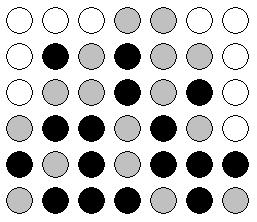
\includegraphics[width=0.25\textwidth]{image/puissance4}
		\end{center}
	%	&
		N.B. : sur ce dessin noir et
		blanc, les jetons rouges apparaissent en noir, les jetons jaunes en
		gris et les cases blanches désignent l'absence de
		jetons. Cet exemple montre une situation du jeu où le joueur «~jaune~»
		est gagnant. En introduisant un jeton dans la
		4\textsuperscript{ème} colonne,
		il a réalisé un alignement de 4 jetons en oblique.
	%\end{supertabular}
	%\end{center}

	
	On demande d’implémenter une classe Puissance4 qui permette de contrôler
	l’état des différentes phases du jeu. Déterminez les attributs de cette
	classe et décrivez-les brièvement de manière à justifier votre choix.
	Dotez ensuite la classe des méthodes permettant de :

	\begin{liste}
		\item 
			savoir si la grille est pleine
		\item 
			mettre la grille à jour lorsque le joueur n (1 ou 2) joue dans la
			colonne j (entre 1 et 7). Cette méthode renverra la valeur booléenne
			faux si la colonne en question est déjà pleine
		\item 
			vérifier si le joueur qui vient de jouer dans la colonne j a gagné la
			partie
	\end{liste}
	
	N.B. : pour la structure qui contiendra le contenu du tableau de jetons,
	on adoptera la convention suivante : 0 pour l’absence de jeton, 1
	représentera un jeton du 1\textsuperscript{er} joueur, et 2 un jeton du
	2\textsuperscript{ème} joueur (on peut donc faire abstraction de la
	couleur du jeton dans ce problème).
\end{Exercice}

\begin{Exercice}{Cartographie}

	Un fichier \code{géo} contient les villes d’un pays avec
	leurs coordonnées dans un plan
	\textit{xy}. Chaque
	enregistrement du fichier contient le nom d’une ville, la position
	\textit{x} (abscisse) et
	\textit{y} (ordonnée). Ces
	positions sont exprimées en kilomètres à partir du coin inférieur
	gauche de la carte.

	Écrire un algorithme qui,
	\textbf{après une seule lecture du
	fichier}, 

	\begin{liste}
		\item
			affiche les noms des deux villes les plus éloignées de ce pays. (On
			suppose qu’il n’y a pas de cas d’ex-aequo)
		\item 
			affiche la liste des villes situées dans un rayon d’au
			plus \textit{r} kilomètres autour
			de la ville maVille
			(\textit{r} et maVille sont des
			paramètres de l’algorithme)
	\end{liste}
	
	Rappel : la distance entre deux
	points
	(\textit{x}\textsubscript{1},
	\textit{y}\textsubscript{1}),
	(\textit{x}\textsubscript{2},
	\textit{y}\textsubscript{2})~d’un
	plan réel est égale à
	\\
	\begin{math}
		\sqrt{{(x_1 - x_2)}^2 + {(y_1 - y_2)}^2}
	\end{math}
\end{Exercice}

\begin{Exercice}{Les congés}
	Les périodes de congés des différents employés d’une firme sont reprises
	dans un tableau booléen \textbf{Congés} bidimensionnel à \textit{n}
	lignes et 366 colonnes. Chaque ligne du tableau correspond à un employé
	et chaque colonne à un jour de l’année. Une case de ce tableau est mise
	à \textbf{vrai} si l’employé correspondant est en congé le jour
	correspondant. La firme en question est opérationnelle 7 jours sur 7,
	on n’y fait donc pas de distinction entre jours ouvrables, week-end et
	jours fériés.

	Ce tableau permet de visualiser l’ensemble des congés des travailleurs,
	et d’accorder ou non une demande de congé, suivant les règles suivantes :

	\begin{enumerate}
		\item 
			une période de congé ne peut excéder 15 jours ;
		\item 
			un employé a droit à maximum 40 jours de congé par an ;
		\item 
			à tout moment, 50\% des employés doivent être présents dans la firme.
	\end{enumerate}
	
	Écrire un algorithme qui détermine si cette demande peut être accordée
	ou non à un employé dont on connait le nom, ainsi que les dates de
	début et de fin d’une demande de congé (objets de la classe Date). Dans
	l’affirmative, le tableau \textbf{Congés} sera mis à jour.

	Pour établir la correspondance entre ce tableau et les noms des
	employés, vous avez à votre disposition un tableau \textbf{Personnel}
	de chaines. L’emplacement du nom d’un employé dans ce tableau
	correspond à l’indice ligne du tableau \textbf{Congés}.

	Il est permis d’utiliser pour résoudre cet exercice la méthode suivante
	de la classe Date, sans devoir détailler son code :
	
	\cadre{
	\begin{pseudo}
		\MethodSign{numéroJour}{}{entier}
		\RComment la position du jour dans l’année (entre 1 et 366)
	\end{pseudo}
	}
\end{Exercice}

\begin{Exercice}{Ruptures et divorces}

Une commune gère la liste de ses couples mariés dans un fichier \code{unions}.
Ce fichier est classé dans l’ordre chronologique des mariages 
et chacun de ses enregistrements, de type \code{Union},
contient les champs suivants :

	\cadre{
	\begin{pseudo}
	\Struct{Union}
	\Decl date : Date \RComment date du mariage
	\Decl nom1 : chaine \RComment nom du premier conjoint
	\Decl num1 : entier \RComment numéro de registre national du premier conjoint
	\Decl nom2 : chaine \RComment nom du second conjoint
	\Decl num2 : entier \RComment numéro de registre national du second conjoint
	\EndStruct
	\end{pseudo}
	}

Les demandes de divorces durant une certaine année 
ont été stockées dans le fichier \code{divorces}
et ses enregistrements sont similaires à ceux de \code{unions} :
chaque enregistrement contient également les noms et numéros des deux
conjoints demandant la séparation, et la date est cette fois-ci celle
du divorce. Le fichier est également classé par ordre chronologique des
demandes de divorces. On peut supposer l’absence d’erreur, c’est-à-dire
que tous les enregistrements de \code{divorces}
ont été répertoriés dans \code{unions}.

Sur base de ces données, écrire \textbf{un} algorithme qui :

\begin{enumerate}
\item {
	crée un fichier \code{unionsUpdate} 
	résultant de la mise à jour du fichier \code{unions}}. 
	Le nouveau fichier ne contiendra plus les couples divorcés 
	renseignées dans le fichier des divorces. 
	Pour comparer les contenus des fichiers en entrée, 
	on se fiera uniquement aux numéros de registre national 
	(car il est possible que des personnes différentes 
	puissent avoir le même nom). 
	Attention, il est possible que les noms des conjoints 
	soient inversés dans \code{divorces}
	par rapport à l’ordre de \code{unions}.
	Veillez aussi à comparer les deux noms 
	avant de supprimer un enregistrement de \code{unions}
	car on peut imaginer le cas de personnes se remariant et divorçant
	plusieurs fois dans l’année !
\item
	donne le mois de l’année où le nombre de divorce a été le plus élevé.
\end{enumerate}

\end{Exercice}

\begin{Exercice}{Le jeu de la vie}

	Le \textbf{jeu de la vie} a été inventé en 1970 
	par le mathématicien anglais John Horton Conway. 
	Ce «~jeu~» ne demandant aucune interaction du «~joueur~» 
	autre que le choix d’une configuration initiale 
	est l’exemple le plus connu d’\textit{automate cellulaire}.

	Il se déroule sur un quadrillage 
	(en théorie infini) dont les carrés, 
	appelés ici \textit{cellules}
	peuvent posséder deux états : 
	ils sont soit \textit{vivants} soit \textit{morts}, 
	ce qui sera respectivement représenté par un carré noir ou blanc. 
	Chaque cellule interagit avec ses 8 cellules voisines 
	(les 8 cellules adjacentes par un coté ou un sommet) 
	et c’est le nombre de cellules avoisinantes qui détermine la naissance, 
	la survie ou la mort d’une cellule d’un stade à l’autre du jeu, 
	appelé \textit{génération}.

	Les règles de vie et de mort des cellules lors du passage d’une
	génération à une autre sont les suivantes :

	\begin{enumerate}
	\item 
		une cellule vivante ayant moins de 2 voisines disparait à la
		génération suivante (mort par isolation)
	\item 
		une cellule vivante ayant plus de 3 voisines disparait à la génération
		suivante (mort par surpopulation)
	\item
		une cellule vivante ayant 2 ou 3 voisines survit à la génération
		suivante
	\item
		une cellule morte entourée de 3 voisines vivantes (re)nait à la
		génération suivante.
	\end{enumerate}

	Le jeu consiste donc simplement à observer l’évolution d’une
	configuration de départ lors des passages successifs d’une génération à
	la suivante. Certaines configurations sont statiques, d’autres
	cycliques, d’autres encore évoluent de manière imprévisible.

	\subsection*{Exemples}

	\subsubsection*{(1) Un oscillateur}

	La configuration de départ est constituée de 3 cellules voisines alignées horizontalement. 
	Les deux cellules extrêmes vont disparaitre, car elles n’ont qu’une seule voisine. 
	La cellule centrale va survivre car elle est entourée de 2 voisines. 
	Les deux cellules mortes marquées d’une croix vont devenir vivantes, 
	de sorte que la configuration à la 2\up{ème} génération 
	sera constituée de 3 cellules alignées verticalement. 
	Par symétrie, la 3\up{ème} génération sera identique à la première, 
	et les générations suivantes formeront donc une situation
	oscillante entre la position horizontale et verticale.

	\begin{footnotesize}
	\sffamily
	\begin{minipage}{0.3\textwidth}
	\begin{center}
	Configuration de départ\\
	\begin{tabular}{|*{6}{>{\centering\arraybackslash}m{0.2cm}|}}
	\hline
	~ & ~ & ~ & ~ & ~ & ~ \\\hline
	~ & ~ & X & ~ & ~ & ~ \\\hline
	~ & \cellcolor{gray!50} & \cellcolor{gray!50} & \cellcolor{gray!50} & ~ & ~ \\\hline
	~ & ~ & X & ~ & ~ & ~ \\\hline
	~ & ~ & ~ & ~ & ~ & ~ \\\hline
	~ & ~ & ~ & ~ & ~ & ~ \\\hline
	\end{tabular}
	\end{center}
	\end{minipage}
	\begin{minipage}{0.3\textwidth}
	\begin{center}
	2\up{ème} génération\\
	\begin{tabular}{|*{6}{>{\centering\arraybackslash}m{0.2cm}|}}
	\hline
	~ & ~ & ~ & ~ & ~ & ~ \\\hline
	~ & ~ & \cellcolor{gray!50} & ~ & ~ & ~ \\\hline
	~ & ~ & \cellcolor{gray!50} & ~ & ~ & ~ \\\hline
	~ & ~ & \cellcolor{gray!50} & ~ & ~ & ~ \\\hline
	~ & ~ & ~ & ~ & ~ & ~ \\\hline
	~ & ~ & ~ & ~ & ~ & ~ \\\hline
	\end{tabular}
	\end{center}
	\end{minipage}
	\begin{minipage}{0.3\textwidth}
	\begin{center}
	3\up{ème} génération\\
	\begin{tabular}{|*{6}{>{\centering\arraybackslash}m{0.2cm}|}}
	\hline
	~ & ~ & ~ & ~ & ~ & ~ \\\hline
	~ & ~ & ~ & ~ & ~ & ~ \\\hline
	~ & \cellcolor{gray!50} & \cellcolor{gray!50} & \cellcolor{gray!50} & ~ & ~ \\\hline
	~ & ~ & ~ & ~ & ~ & ~ \\\hline
	~ & ~ & ~ & ~ & ~ & ~ \\\hline
	~ & ~ & ~ & ~ & ~ & ~ \\\hline
	\end{tabular}
	\end{center}
	\end{minipage}
	\end{footnotesize}

	\subsubsection*{(2) Le vaisseau spatial}

	Dans cet exemple, le motif de 5 cellules retrouve sa forme initiale
	toutes les 4 générations, mais s’est déplacé d’une position en
	direction diagonale.

	\begin{center}
	\begin{footnotesize}
	\sffamily
	\begin{minipage}{0.3\textwidth}
	\begin{center}
	départ\\
	\begin{tabular}{|*{6}{>{\centering\arraybackslash}m{0.2cm}|}}
	\hline
	~ & ~ & ~ & ~ & ~ & ~ \\\hline
	~ & ~ & \cellcolor{gray!50} & ~ & ~ & ~ \\\hline
	~ & ~ & ~ & \cellcolor{gray!50} & ~ & ~ \\\hline
	~ & \cellcolor{gray!50} & \cellcolor{gray!50} & \cellcolor{gray!50} & ~ & ~ \\\hline
	~ & ~ & ~ & ~ & ~ & ~ \\\hline
	~ & ~ & ~ & ~ & ~ & ~ \\\hline
	\end{tabular}
	\end{center}
	\end{minipage}
	\begin{minipage}{0.3\textwidth}
	\begin{center}
	2\up{ème} génération\\
	\begin{tabular}{|*{6}{>{\centering\arraybackslash}m{0.2cm}|}}
	\hline
	~ & ~ & ~ & ~ & ~ & ~ \\\hline
	~ & ~ & ~ & ~ & ~ & ~ \\\hline
	~ & \cellcolor{gray!50} & ~ & \cellcolor{gray!50} & ~ & ~ \\\hline
	~ & ~ & \cellcolor{gray!50} & \cellcolor{gray!50} & ~ & ~ \\\hline
	~ & ~ & \cellcolor{gray!50} & ~ & ~ & ~ \\\hline
	~ & ~ & ~ & ~ & ~ & ~ \\\hline
	\end{tabular}
	\end{center}
	\end{minipage}
	\begin{minipage}{0.3\textwidth}
	\begin{center}
	3\up{ème} génération\\
	\begin{tabular}{|*{6}{>{\centering\arraybackslash}m{0.2cm}|}}
	\hline
	~ & ~ & ~ & ~ & ~ & ~ \\\hline
	~ & ~ & ~ & ~ & ~ & ~ \\\hline
	~ & ~ & ~ & \cellcolor{gray!50} & ~ & ~ \\\hline
	~ & \cellcolor{gray!50} & ~ & \cellcolor{gray!50} & ~ & ~ \\\hline
	~ & ~ & \cellcolor{gray!50} & \cellcolor{gray!50} & ~ & ~ \\\hline
	~ & ~ & ~ & ~ & ~ & ~ \\\hline
	\end{tabular}
	\end{center}
	\end{minipage}
	\end{footnotesize}
	\end{center}
	
	\begin{center}
	\begin{footnotesize}
	\sffamily
	\begin{minipage}{0.3\textwidth}
	\begin{center}
	4\up{ème} génération\\
	\begin{tabular}{|*{6}{>{\centering\arraybackslash}m{0.2cm}|}}
	\hline
	~ & ~ & ~ & ~ & ~ & ~ \\\hline
	~ & ~ & ~ & ~ & ~ & ~ \\\hline
	~ & ~ & \cellcolor{gray!50} & ~ & ~ & ~ \\\hline
	~ & ~ & ~ & \cellcolor{gray!50} & \cellcolor{gray!50} & ~ \\\hline
	~ & ~ & \cellcolor{gray!50} & \cellcolor{gray!50} & ~ & ~ \\\hline
	~ & ~ & ~ & ~ & ~ & ~ \\\hline
	\end{tabular}
	\end{center}
	\end{minipage}
	\begin{minipage}{0.3\textwidth}
	\begin{center}
	5\up{ème} génération\\
	\begin{tabular}{|*{6}{>{\centering\arraybackslash}m{0.2cm}|}}
	\hline
	~ & ~ & ~ & ~ & ~ & ~ \\\hline
	~ & ~ & ~ & ~ & ~ & ~ \\\hline
	~ & ~ & ~ & \cellcolor{gray!50} & ~ & ~ \\\hline
	~ & ~ & ~ & ~ & \cellcolor{gray!50} & ~ \\\hline
	~ & ~ & \cellcolor{gray!50} & \cellcolor{gray!50} & \cellcolor{gray!50} & ~ \\\hline
	~ & ~ & ~ & ~ & ~ & ~ \\\hline
	\end{tabular}
	\end{center}
	\end{minipage}
	\end{footnotesize}
	\end{center}
	
	\bigskip

	On veut créer une classe permettant d’implémenter 
	la représentation du jeu de la vie sur un tableau à deux
	dimensions possédant un nombre $n$ de lignes et $m$ de colonnes, 
	les éléments de ce tableau étant des booléens 
	(vrai pour une cellule vivante et faux pour une cellule morte).
	
	On voudrait doter cette classe de méthodes permettant :

	\begin{enumerate}
	\item 
		de créer une configuration initiale à partir
		d’un fichier \code{init} de \code{Couples}
		(structure constituée de deux entiers). 
		Le premier enregistrement du fichier donnerait les dimensions du tableau,
		et les suivants donneraient les coordonnées des cases vivantes de la
		configuration initiale.
		
		Par exemple, les couples du fichier \code{init} pour le vaisseau spatial
		seraient : (6,6), (2,3), (3,4), (4,2), (4,3), (4,4). Le premier couple
		donne donc les dimensions du tableau (6~x~6) et les 5 suivants les
		coordonnées des 5 cellules vivantes.
	\item 
		de connaitre le nombre de cellules vivantes de la génération en cours
	\item
		de passer à la génération suivante ; cette méthode remplace donc le
		tableau représentant une génération par le tableau représentant la
		génération suivante
	\item
		de connaitre le nombre de cellules qui seront
		vivantes $k$ générations plus tard
		($k$ étant un paramètre entier). 
		Attention, cette méthode ne doit pas perdre la configuration de la génération courante.
	\end{enumerate}

	\subsubsection*{N.B. :}

	\begin{liste}
	\item
		Veillez à prendre vos dispositions pour ne pas recopier deux fois le
		code apparaissant dans les méthodes 3 et 4 !
	\item
		Astuce pour simplifier votre algorithme : 
		on peut considérer que le bord du tableau est encore entouré 
		d’une couche de cellules mortes 
		– aucune d’elles ne prend donc naissance, même si un alignement de 3 cellules
		vivantes se trouve sur le bord du tableau visible. 
		Il suffit pour cela d’utiliser un tableau indicé de $0$ à $n+1$ pour les lignes 
		et de $0$ à $m+1$ pour les colonnes, 
		avec comme conséquence que le traitement des $m$ x $n$ cases centrales 
		sera identique pour chaque case.
	\end{liste}

\end{Exercice}

\begin{Exercice}{Messages codés}

{
L'agent ESI 007 a imaginé un nouveau procédé de codage
de ses messages secrets. Celui-ci fonctionne en trois étapes. La
première consiste à remplacer chaque lettre du message par la lettre se
trouvant un certain nombre de positions plus loin dans l’alphabet, ce
nombre de positions étant égal à la longueur du mot ! Ainsi,}

{\centering
RENDEZ VOUS A 10 HEURES A L’ ESI
\par}

{
deviendra}

{\centering
XKTJKF ZSYW B 10 NKAXKY \ B M’ HVL
\par}

{
En effet, toutes les lettres de RENDEZ et de HEURES (mots de longueur 6)
ont été décalées de 6 positions dans l’alphabet ; noter que le décalage
est cyclique, la lettre Z ayant été remplacée par F et U par A. De
même, toutes les lettres de VOUS (de longueur 4) ont été décalées de 4
positions, A est devenu B et L est devenu M (puisque ces mots sont de
longueur 1) et enfin, les lettres d’ESI (de longueur 3) ont été
décalées de 3 positions. Notez que seules les lettres sont modifiées,
les autres caractères sont inchangés (chiffres, ponctuation,
guillemets, etc.)}

{
Pour la seconde étape, ESI 007 brouille les pistes en intercalant en
troisième position une lettre choisie aléatoirement, mais seulement
dans les mots \textbf{d’au moins 4 lettres}. Cela donne par exemple
pour le message précédent :}

{\centering
XKETJKF ZSQYW B 10 NKDAXKY B M’ HVL
\par}

{
(Avouez que le message de départ est déjà bien méconnaissable…). Enfin,
le message obtenu après cette seconde étape est caché dans un fichier
\textbf{SECRET} dont chaque enregistrement correspond à un mot du
message codé, et contient les champs suivant :}

\begin{liste}
\item {
id : «~indice début~» : entier}
\item {
if : «~indice fin~» : entier}
\item {
tabCar : tableau[1 à 20] de caractère qui représente un des mots du
message codé. Ce mot se trouve entre les éléments d’indices ID et IF
inclus, les autres éléments du tableau sont choisis aléatoirement.}
\end{liste}
{
Pour fixer les idées, le premier enregistrement de SECRET pourrait être
:}

\begin{center}
\begin{tabular}{*{1}{>{\small\centering\arraybackslash}m{0.35cm}}}
id \\
8\\
\end{tabular}
\begin{tabular}{*{1}{>{\small\centering\arraybackslash}m{0.35cm}}}
if\\
14\\
\end{tabular}
\begin{tabular}{*{20}{>{\small\centering\arraybackslash}m{0.32cm}}}
\multicolumn{4}{l}{tabCar} \\
F & A & 3 & P & Y & ! & R & K & K & E & T & J & K & F & R & Z & ; & C & W & J \\
\end{tabular}
\end{center}

On retrouve en effet entre les éléments d’indice 8 et 14 le premier mot
codé du message «~\textit{XKETJKF~}». On peut supposer que dans tous
les cas, 1 ${\leq}$ id ${\leq}$ if ${\leq}$ 20.

Connaissant le procédé de cryptage d’ESI 007, on vous demande d’écrire
un algorithme qui \textbf{décrypte} un message crypté par cette
méthode. Les lettres du message \textbf{décrypté} seront écrites une
par une dans le fichier \code{lisezMoi} (en n’oubliant pas de séparer les
mots par un caractère blanc !). 
\end{Exercice}
